% !TeX root = sections.tex
\graphicspath{{figures/}}

{\bf Spherical Harmonics}

The set of shperical harmonics is an orthonormal set of functions defined in the unit sphere. They are given as the angular part of the solution to the Laplace Equation in spherical coordinates. Analogously  to how sines and cosines are used in harmonic analysis to represent periodic functions through Fourier Series, Spherical Harmonics may be used to define functions in the surface of a sphere.

{\bf Spherical Coordinates}

It is important to identify the coordinates to be used, as, for instance, spherical coordinates have often two different interpretations: one, which is mainly used by mathematicians, uses the latitude, being the angle between the position vector and the equatorial plane, as one of the angular coordinates; while the other, broadly employed by physicists, uses the co-latitude, defined as the angle between the position vector and the $z$ axis, thus being the complementary of the latitude. 

Here, the spherical coordinates are taken to be
\begin{itemize} 
\item[] $r$, the radial distance from Earth's centre
\item[] $\phi$, the East longitude, bounded between $-\pi$ and $\pi$
\item[] $\theta$, the co-latitude, defined to be $\theta = \frac{\pi}{2} - \theta'$, with $\theta'$ the latitude. $\theta \in \left[0,\pi\right]$ %Bounded between $0$ and $\pi$
\end{itemize}

The magnetic field is given by the negative gradient of the potential $V$ defined for $r \geq R_e$, and given by the spherical harmonic approximation

\begin{equation} \label{eq:igrf_potential}
V = r \sum_{n=1}^{L} \left(\dfrac{R_e}{r}\right)^{n+1} \sum_{m=0}^{n} \left(g_n^m cos(m\phi) + h_n^m sin(m\phi)\right) P_n^m(cos\theta)
\end{equation}

That is
\begin{equation}
{\bm \beta} = -\nabla V
\end{equation}

Where $g_n^m$ and $h_n^m$ are the set of IGRF gaussian coefficients, published and revised every five years by the participating members of the IAGA (International Association
of Geomagnetism and Aeronomy). The $12^{th}$ generation is here used, as the last revision by the time of this work. These coefficient also include the secular variation (SV), which bestow the model on the proper time dependence. Keping track of the change in the coefficients in $nT$ per year. The coefficients  for some epoch year are referred to as IGRF. When real data about the geomagnetic field becomes available so that some adjustements can be made, the model becomes definitive and changes its name to DGRF (Deffinitive geomagnetic reference field).

$P_n^m(cos \theta)$ are the Schmidt normalized associated Legendre polynomials of degree n and order m

One can find very effective, recursive ways of computing the Schmidt quasi-normalization factors, the Associated Legendre polynomials and its derivatives, as can be found on [J.Davis - Mathematical Modeling of Earth’s Magnetic Field] %\cite{...}

The three components of the magnetic field in $r$, $\phi$ and $\theta$ directions can be found in terms of the partial derivatives of \ref{eq:igrf_potential}


\begin{equation} \label{eq:local_sph_cpmt}
\begin{aligned}
{\bm \beta}_r &= -\dfrac{\partial V}{\partial r} = \sum_{n=1}^{N} (n+1) \left(\dfrac{R_e}{r}\right)^{n+2} \sum_{m=0}^{n} \left(g_n^m cos(m\phi) + h_n^m sin(m\phi)\right) P_n^m(\theta)\\
{\bm \beta}_{\theta} &= -\dfrac{1}{r} \dfrac{\partial V}{\partial \theta} = 
-\sum_{n=1}^{L} \left(\dfrac{R_e}{r}\right)^{n+2} \sum_{m=0}^{n} \left(g_n^m cos(m\phi) + h_n^m sin(m\phi)\right) \dfrac{\partial P_n^m(\theta)}{\partial \theta}\\
{\bm \beta}_{\phi} &= -\dfrac{1}{r sin\theta} \dfrac{\partial V}{\partial \phi} = 
\dfrac{1}{sin\phi}\sum_{n=1}^{L} \left(\dfrac{R_e}{r}\right)^{n+2} \sum_{m=0}^{n} m\left(g_n^m sin(m\phi) - h_n^m cos(m\phi)\right) P_n^m(\theta)
\end{aligned}
\end{equation}


{\bf Legendre Polynomials}

The set of regular Legendre Polynomials is given by the solutions $P_n(\nu)$ to the equation
\begin{equation}
\dfrac{1}{\sqrt{1-2\nu x + x^2}} = \sum_{n=0}^\infty x^2 P_n(\nu)
\end{equation}
Which gives
\begin{equation}
P_n(\nu) = \dfrac{1}{n! 2^n} \dfrac{d^n}{d\nu^n} (\nu^2 -1)^n
\end{equation}

{\bf Associated Legendre Polynomials}

The associated Legendre polynomials $P_n^m(\nu)$ of degree n and order m relate to $P_n(\nu)$ by
\begin{equation}
P_{n,m}(\nu) = (1-\nu^2)^{\frac{1}{2m}} \dfrac{d^m}{d\nu^m}(P_n(\nu))
\end{equation}
These polynomials are not normalized in any way. %Not too sure about this sentence
Recall that, in order to use the spherical harmonic approximation, one needs to find the Schmidt quasi-normalization of the corresponding Legendre Polynomials. Such approximation is derived in what follows.

{\bf Gaussian normalization and Schmidt quasi-normalization}
The two most broadly used normalizations are the Gaussian normalization and the Schmidt quasi-normalization (see, for instance [R. A. Langel. Geomagnetism]).
To compute the geomagnetic field, the Schmidt quasi-normalization is used, and it relates to the associated Legendre Polynomials by
\begin{equation}
P_n^m(\nu) = \sqrt{\dfrac{2(n-m)!}{(n+m)!}} P_{n,m}(\nu) 
\end{equation}

However, it is much more efficient to compute the Gaussian normalized Legendre polynomials $P^{n,m}$, whose interest lies in the existence of a recursive formula for their effective computation [James R.Wertz. Spacecraft Attitude Determination and Control]. These are given by
\begin{equation}
P^{n,m}(\nu) = \dfrac{2^n! (n-m)!}{(2n)!} P_{n,m}(\nu)
\end{equation}

An can be related to the Schmidt quasi-normalized Legendre Polynomials by using
\begin{equation}
P_n^m(\nu) = \Gamma_{n,m} P^{n,m}(\nu)
\end{equation}
Where
\begin{equation}
\begin{aligned}
\Gamma_{n,m} &= \sqrt{\dfrac{(n-m)!}{(n+m)!}}\dfrac{(2n-1)!!}{(n-m)!}, &m = 0\\
\Gamma_{n,m} &= \sqrt{\dfrac{2(n-m)!}{(n+m)!}}\dfrac{(2n-1)!!}{(n-m)!}, &m \neq 0
\end{aligned}
\end{equation}

The algorithm will calculate, for a given value of $\theta$, the Gaussian normalized Legendre Polynomials $P^{n,m}(\theta)$ and its derivatives $\dfrac{d^m}{d\nu^m}(P^{n,m}(\nu))$, using the recursive formulas presented by [James R.Wertz. Spacecraft Attitude Determination and Control], and outlined below.

One step further, it is computationally cheaper to modify the IGRF coefficients, using the relation
\begin{equation}
\begin{aligned}
g_{n,m} &= \Gamma_{n,m}\ g_n^m \\ h_{n,m} &= \Gamma_{n,m}\  h_n^m
\end{aligned}
\end{equation}

So that the recursive algorithm for the Schmidt quasi-normalization coefficients ([James R.Wertz. Spacecraft Attitude Determination and Control]) is ran only once for each pair $(m,n)$.

\textbf{Transformation to inertial reference frame}

After the three components of the magnetic field $\beta_r$, $\beta_{\theta}$ and $\beta_{\phi}$ from ()\ref{eq:local_sph_cpmt}) in local spherical coordinates are calculated, we aim to express them in terms of an Earth centred inertial reference frame. This transformation is given by \ref{eq:transf_magnt}, and it is illustrated in figure~\ref{fig:transf_magnt}

\begin{equation}
\begin{aligned} \label{eq:transf_magnt}
\beta_x &= \left(\beta_r cos(\theta') +  \beta_{\theta}sin(\theta')\right)cos(l) - \beta_{\phi}sin(l)\\
\beta_y &= \left(\beta_r cos(\theta') +  \beta_{\theta}sin(\theta')\right)sin(l) + \beta_{\phi}cos(l)\\
\beta_z &= \beta_r sin(\theta') + \beta_{\theta} cos(l)
\end{aligned}
\end{equation}

\begin{figure} \label{fig:transf_magnt}
	\centering
	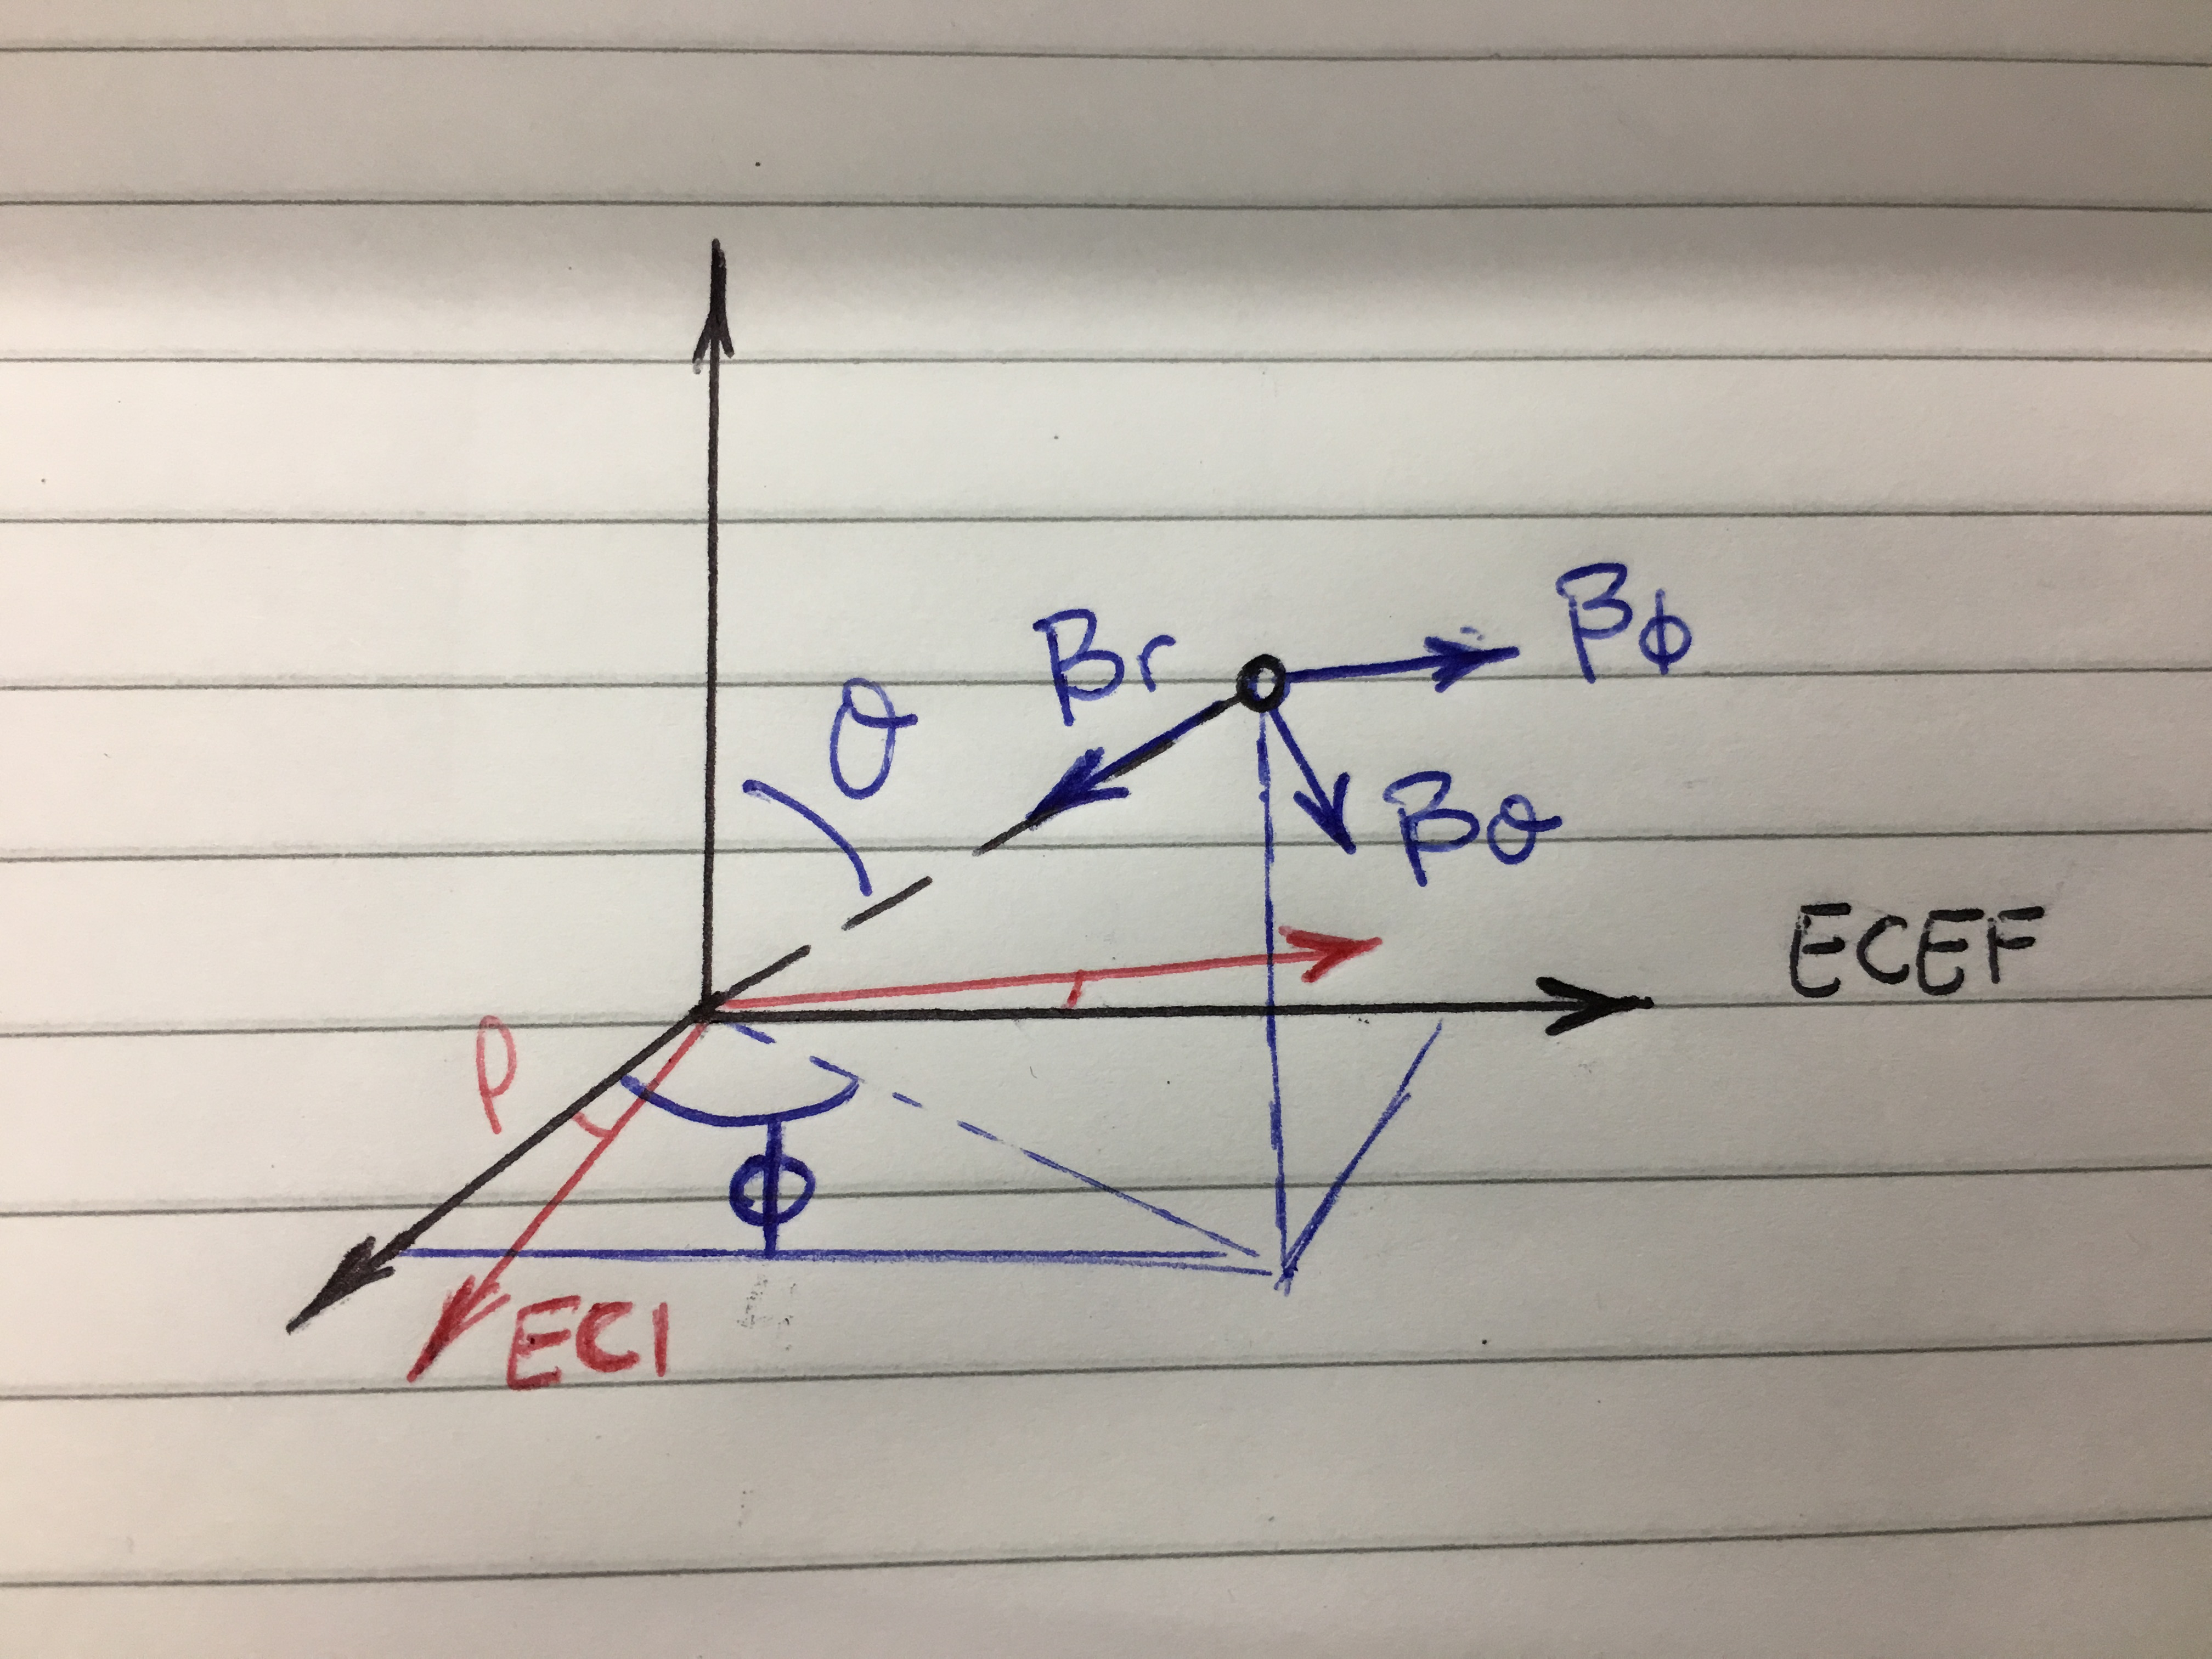
\includegraphics[width=0.4\textheight]{frame_transformation_magnetic_tmp.jpeg}
	\caption{Frame transformation between local spherical and inertial reference frame}
\end{figure}

{\bf Recursive formulas for Gaussian normalized Legendre polynomials, its derivatives and Schmidt quasi-normalization factors}

{\it Associated Legendre polynomials and derivatives}
\begin{equation} \label{eq:Legendre_Recursive}
\begin{aligned}
P^{0,0}(\theta) &= 1\\
P^{n,m}(\theta) &= sin(\theta)P^{n-1,m-1}\\
P^{n,m}(\theta) &= cos(\theta)P^{n-1,m} - K^{n,m}P^{n-2,m}
\end{aligned}
\end{equation}

\begin{equation} \label{eq:dLegendre_Recursive}
\begin{aligned}
\dfrac{\partial P^{0,0}(\theta)}{\partial \theta} &= 0\\
\dfrac{\partial P^{n,n}(\theta)}{\partial \theta} &= sin(\theta)\dfrac{\partial P^{n-1,n-1}(\theta)}{\partial \theta} + cos(\theta)P^{n-1,n-1}\\
\dfrac{\partial P^{n,m}(\theta)}{\partial \theta} &= cos(\theta)\dfrac{\partial P^{n-1,m}(\theta)}{\partial \theta} - sin(\theta)P^{n-1,m} - K^{n,m}\dfrac{\partial P^{n-2,m}(\theta)}{\partial \theta}
\end{aligned}
\end{equation}


{\it Schmidt quasi-normalization factors}
\begin{equation}
\begin{aligned}
\Gamma_{0,0} &= 1\\
\Gamma_{n,0} &= \dfrac{2n-1}{n}\Gamma_{n-1,0}\\
\Gamma_{n,m} &= \sqrt{\dfrac{(n-m+1)(\delta_m^1+1)}{n+m}}\Gamma_{n,m-1}
\end{aligned}
\end{equation}


\footnote{Note the use of upper and subscript notation here to distinguish between Regular, Associated, and Schmidt quasi-normalized Legendre polynomials}

